\chapter{Introduzione ai Container}

\section*{Introduzione}
I container rappresentano una rivoluzione nel modo in cui sviluppiamo, distribuiamo ed eseguiamo applicazioni. Questo capitolo introduce i concetti fondamentali della containerizzazione, le differenze con le macchine virtuali tradizionali e l'architettura di Docker.

\section*{Obiettivi di apprendimento}
\begin{itemize}
    \item Comprendere cosa sono i container e come funzionano
    \item Confrontare container e macchine virtuali
    \item Conoscere i vantaggi della containerizzazione
    \item Capire l'architettura di Docker e i suoi componenti
    \item Identificare i casi d'uso appropriati per i container
\end{itemize}

\section{Cos'è un Container?}

\subsection{Definizione}
Un \textbf{container} è un'unità software standardizzata che impacchetta il codice e tutte le sue dipendenze in modo che l'applicazione possa essere eseguita in modo rapido e affidabile da un ambiente di computing a un altro.

\begin{tcolorbox}[colback=blue!10, colframe=blue!60, title=Analogia: Container di Spedizione]
Come i container di spedizione standardizzano il trasporto merci, i container software standardizzano il deployment di applicazioni:
\begin{itemize}
    \item \textbf{Dimensioni standard}: Formato uniforme e prevedibile
    \item \textbf{Portabilità}: Si spostano facilmente tra navi, treni, camion
    \item \textbf{Isolamento}: Il contenuto è separato dall'esterno
    \item \textbf{Efficienza}: Caricamento/scaricamento ottimizzato
\end{itemize}
\end{tcolorbox}

\subsection{Caratteristiche principali}

I container Docker si caratterizzano per un insieme di proprietà che li rendono particolarmente adatti agli ambienti di sviluppo e produzione moderni. L'\textbf{isolamento} costituisce una delle caratteristiche fondamentali: ogni container opera con il proprio filesystem dedicato, gestisce i propri processi in modo indipendente e dispone di un proprio stack di networking, garantendo così che le applicazioni non interferiscano tra loro.

La \textbf{portabilità} è espressa efficacemente dal motto "Build once, run anywhere": un container costruito su un sistema può essere eseguito senza modifiche su qualsiasi piattaforma che supporti Docker, eliminando i problemi di compatibilità tra ambienti diversi. La \textbf{leggerezza} deriva dalla condivisione del kernel dell'host, che permette ai container di avviarsi in pochi secondi e di occupare solo lo spazio necessario per l'applicazione e le sue dipendenze, senza il sovraccarico di un sistema operativo completo.

L'\textbf{immutabilità} garantisce che l'immagine del container rimanga invariata durante il suo ciclo di vita, assicurando deployment consistenti e riproducibili. Infine, la \textbf{scalabilità} è intrinseca all'architettura dei container: possono essere facilmente replicati per distribuire il carico di lavoro, permettendo alle applicazioni di adattarsi dinamicamente alle esigenze di traffico e computazione.

\section{Container vs Macchine Virtuali}

\subsection{Architettura a confronto}

\begin{figure}[h]
    \centering
    \begin{tikzpicture}[
        box/.style={rectangle, draw, minimum width=3cm, minimum height=0.8cm, align=center},
        layer/.style={box, fill=blue!20},
        vm/.style={box, fill=green!20},
        container/.style={box, fill=orange!20}
    ]
        % Virtual Machines
        \node[layer] (hw1) at (0,0) {Hardware};
        \node[layer] (os1) at (0,1) {OS Host};
        \node[layer] (hyp) at (0,2) {Hypervisor};
        \node[vm] (gos1) at (-1.5,3) {Guest OS};
        \node[vm] (gos2) at (0,3) {Guest OS};
        \node[vm] (gos3) at (1.5,3) {Guest OS};
        \node[vm] (app1) at (-1.5,4) {App A};
        \node[vm] (app2) at (0,4) {App B};
        \node[vm] (app3) at (1.5,4) {App C};

        \node[above=0.3cm of app2] {\textbf{Virtual Machines}};

        % Containers
        \node[layer] (hw2) at (6,0) {Hardware};
        \node[layer] (os2) at (6,1) {OS Host};
        \node[layer] (docker) at (6,2) {Docker Engine};
        \node[container] (cnt1) at (4.5,3.5) {App A\\Libs};
        \node[container] (cnt2) at (6,3.5) {App B\\Libs};
        \node[container] (cnt3) at (7.5,3.5) {App C\\Libs};

        \node[above=0.3cm of cnt2] {\textbf{Containers}};
    \end{tikzpicture}
    \caption{Architettura: Virtual Machines vs Containers}
\end{figure}

\subsection{Differenze chiave}

\begin{table}[h]
\centering
\begin{tabular}{|l|l|l|}
\hline
\textbf{Caratteristica} & \textbf{Virtual Machine} & \textbf{Container} \\
\hline
Dimensione & GB (include intero OS) & MB (solo app + dipendenze) \\
Avvio & Minuti & Secondi \\
Performance & Overhead hypervisor & Quasi native \\
Isolamento & Completo (hardware) & A livello processo \\
Portabilità & Limitata (formato VM) & Eccellente (standard OCI) \\
Densità & Decine per host & Centinaia per host \\
\hline
\end{tabular}
\caption{Confronto VM vs Container}
\end{table}

\subsection{Virtual Machines}

Le macchine virtuali rappresentano un approccio consolidato alla virtualizzazione, con caratteristiche distintive che le rendono appropriate per scenari specifici. L'\textbf{isolamento completo a livello hardware} costituisce il vantaggio principale: ogni VM opera con risorse completamente separate, garantendo che problemi in una VM non possano propagarsi ad altre. La capacità di eseguire \textbf{sistemi operativi diversi sullo stesso host} offre flessibilità massima: è possibile far convivere Windows, Linux e altri OS su una singola macchina fisica. La \textbf{sicurezza superiore}, assicurata dalla separazione fornita dall'hypervisor, rende le VM ideali per ambienti multi-tenant. Infine, il \textbf{supporto per applicazioni legacy} permette di mantenere in esecuzione software datato che richiede specifiche configurazioni OS.

Questi vantaggi comportano però costi considerevoli. L'\textbf{overhead significativo} deriva dal fatto che ogni VM include un sistema operativo completo, consumando gigabyte di spazio e memoria anche per applicazioni minime. L'\textbf{avvio lento} è inevitabile: il boot di un intero sistema operativo richiede tipicamente diversi minuti, rallentando le operazioni di deployment e scaling. Il \textbf{consumo elevato di risorse}---RAM, CPU e disco---limita drasticamente il numero di istanze eseguibili su un singolo server fisico. La \textbf{portabilità limitata tra hypervisor diversi} crea lock-in tecnologico: migrare VM tra VMware, KVM o Hyper-V può richiedere conversioni complesse.

\subsection{Containers}

I container rappresentano un cambiamento paradigmatico rispetto alle VM, con vantaggi pronunciati in termini di efficienza ed agilità. La \textbf{leggerezza} deriva dalla condivisione del kernel dell'host: i container includono solo l'applicazione e le sue dipendenze dirette, eliminando la duplicazione del sistema operativo. L'\textbf{avvio istantaneo}, misurato in secondi anziché minuti, accelera drammaticamente i cicli di deployment e scaling. L'\textbf{alta densità} permette di eseguire centinaia di container su un singolo server, massimizzando l'utilizzo dell'hardware. La \textbf{portabilità} è eccezionale: un container funziona identicamente su qualsiasi sistema con Docker, dalla workstation dello sviluppatore ai datacenter cloud. L'\textbf{efficienza} si manifesta nel minor spreco di risorse, con CPU e memoria allocate solo dove necessario. L'\textbf{integrazione CI/CD} è naturale: i container si inseriscono perfettamente nelle pipeline DevOps moderne, automatizzando build, test e deployment.

Tuttavia, i container presentano limitazioni intrinseche alla loro architettura. L'\textbf{isolamento meno robusto} rispetto alle VM deriva dalla condivisione del kernel: la separazione avviene a livello processo, non hardware. La necessità di utilizzare lo \textbf{stesso kernel dell'host} impedisce l'esecuzione di sistemi operativi diversi: un host Linux può ospitare solo container Linux. Dal punto di vista della \textbf{sicurezza}, una vulnerabilità nel kernel condiviso può teoricamente compromettere tutti i container in esecuzione. Infine, i container \textbf{non sono adatti per applicazioni che richiedono un kernel diverso} o modifiche a livello sistema, limitandone l'applicabilità in alcuni contesti specializzati.

\begin{nota}
Container e VM non sono mutualmente esclusivi. Molte architetture moderne usano \textbf{container dentro VM}: le VM forniscono isolamento hardware, i container portano portabilità e densità.
\end{nota}

\section{Vantaggi della Containerizzazione}

\subsection{1. Portabilità e Consistenza}

\begin{tcolorbox}[colback=green!10, colframe=green!60, title=Problema: "Works on my machine"]
\textbf{Scenario tradizionale}:
\begin{itemize}
    \item Sviluppo su macOS
    \item Staging su Ubuntu 20.04
    \item Produzione su CentOS 8
    \item Risultato: bug dipendenti dall'ambiente
\end{itemize}

\textbf{Soluzione con container}:
\begin{itemize}
    \item Immagine Docker identica ovunque
    \item Stesso runtime, librerie, dipendenze
    \item Risultato: comportamento prevedibile
\end{itemize}
\end{tcolorbox}

\subsection{2. Microservizi e Scalabilità}

I container si rivelano la tecnologia ideale per implementare architetture a microservizi moderne. L'\textbf{isolamento} intrinseco permette di incapsulare ogni servizio in un container separato, con le sue dipendenze specifiche senza conflitti con altri componenti. La \textbf{scalabilità indipendente} rappresenta un vantaggio cruciale: è possibile aumentare le repliche solo dei servizi sotto carico, ottimizzando l'utilizzo delle risorse senza dover scalare l'intera applicazione monolitica. Il \textbf{deployment incrementale} diventa naturale: ogni microservizio può essere aggiornato indipendentemente, permettendo rilasci frequenti senza downtime dell'intero sistema. La \textbf{resilienza} del sistema migliora significativamente: il fallimento di un singolo container può essere gestito automaticamente con restart o replica su altra macchina, senza compromettere i servizi rimanenti.

\begin{lstlisting}[caption=Esempio: Stack microservizi]
# Frontend
Container 1: React app (3 repliche)

# Backend API
Container 2: Node.js API (5 repliche)
Container 3: Python ML service (2 repliche)

# Database
Container 4: PostgreSQL (1 replica master)
Container 5: Redis cache (2 repliche)
\end{lstlisting}

\subsection{3. DevOps e CI/CD}

I container accelerano il ciclo di sviluppo:

\begin{enumerate}
    \item \textbf{Sviluppo}: Ambiente identico per tutti i developer
    \item \textbf{Testing}: Test automatici in container isolati
    \item \textbf{Build}: Immagine Docker come artifact immutabile
    \item \textbf{Deployment}: Push immagine su registry, pull in produzione
    \item \textbf{Rollback}: Ritorna alla versione precedente in secondi
\end{enumerate}

\begin{figure}[h]
    \centering
    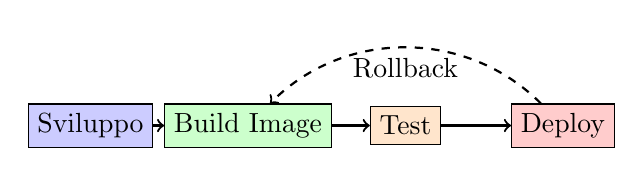
\begin{tikzpicture}[node distance=2cm]
        \node[draw, rectangle, fill=blue!20] (dev) {Sviluppo};
        \node[draw, rectangle, fill=green!20, right of=dev] (build) {Build Image};
        \node[draw, rectangle, fill=orange!20, right of=build] (test) {Test};
        \node[draw, rectangle, fill=red!20, right of=test] (deploy) {Deploy};

        \draw[->, thick] (dev) -- (build);
        \draw[->, thick] (build) -- (test);
        \draw[->, thick] (test) -- (deploy);
        \draw[->, thick, dashed] (deploy) to[bend right=45] node[below] {Rollback} (build);
    \end{tikzpicture}
    \caption{Pipeline CI/CD con Docker}
\end{figure}

\subsection{4. Efficienza delle Risorse}

\begin{table}[h]
\centering
\begin{tabular}{|l|r|r|r|}
\hline
\textbf{Metrica} & \textbf{VM} & \textbf{Container} & \textbf{Risparmio} \\
\hline
Memoria per istanza & 2 GB & 100 MB & 95\% \\
Tempo avvio & 60 sec & 2 sec & 97\% \\
Istanze per server & 10 & 100 & 10x \\
Costo cloud mensile & \$500 & \$50 & 90\% \\
\hline
\end{tabular}
\caption{Confronto efficienza risorse (valori medi)}
\end{table}

\section{Architettura Docker}

\subsection{Componenti principali}

\begin{figure}[h]
    \centering
    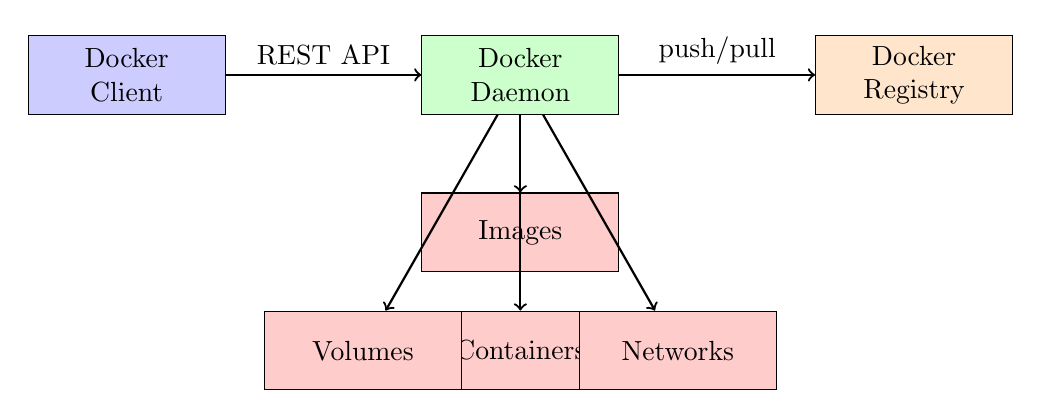
\begin{tikzpicture}[
        component/.style={rectangle, draw, minimum width=2.5cm, minimum height=1cm, align=center},
        arrow/.style={->, thick}
    ]
        % Docker Client
        \node[component, fill=blue!20] (client) at (0,0) {Docker\\Client};

        % Docker Daemon
        \node[component, fill=green!20] (daemon) at (5,0) {Docker\\Daemon};

        % Registry
        \node[component, fill=orange!20] (registry) at (10,0) {Docker\\Registry};

        % Objects
        \node[component, fill=red!20] (images) at (5,-2) {Images};
        \node[component, fill=red!20] (containers) at (5,-3.5) {Containers};
        \node[component, fill=red!20] (volumes) at (3,-3.5) {Volumes};
        \node[component, fill=red!20] (networks) at (7,-3.5) {Networks};

        % Arrows
        \draw[arrow] (client) -- node[above] {REST API} (daemon);
        \draw[arrow] (daemon) -- node[above] {push/pull} (registry);
        \draw[arrow] (daemon) -- (images);
        \draw[arrow] (daemon) -- (containers);
        \draw[arrow] (daemon) -- (volumes);
        \draw[arrow] (daemon) -- (networks);
    \end{tikzpicture}
    \caption{Architettura Docker}
\end{figure}

\subsubsection{Docker Client}

Il Docker Client costituisce l'interfaccia principale attraverso cui gli utenti interagiscono con Docker. Il comando \texttt{docker} fornisce la CLI (Command Line Interface) completa per tutte le operazioni, dalla gestione delle immagini all'esecuzione dei container. Internamente, il client comunica con il Docker Daemon tramite REST API, permettendo un'architettura distribuita in cui il client può connettersi anche a daemon remoti, facilitando la gestione di infrastrutture Docker multi-host.

\begin{lstlisting}[language=bash]
# Esempi di comandi client
$ docker run nginx
$ docker ps
$ docker build -t myapp .
$ docker push myapp:latest
\end{lstlisting}

\subsubsection{Docker Daemon (dockerd)}

Il Docker Daemon rappresenta il cuore pulsante del sistema Docker, operando come processo in background che orchestra tutte le operazioni fondamentali. Si occupa del ciclo di vita completo dei container: building, running e distributing. Gestisce centralmente tutti gli oggetti Docker---immagini, container, reti e volumi---mantenendo lo stato del sistema e garantendo la coerenza delle operazioni. Comunica con i registry esterni per operazioni di push e pull delle immagini, fungendo da intermediario tra lo storage locale e i repository remoti. Espone una REST API completa che permette ai client di inviare comandi e ricevere risposte, abilitando sia l'uso interattivo che l'automazione programmatica.

\subsubsection{Docker Registry}

Un Docker Registry è un sistema di storage e distribuzione per immagini Docker, essenziale per condividere e distribuire applicazioni containerizzate. \textbf{Docker Hub} rappresenta il registry pubblico ufficiale, ospitando milioni di immagini sia ufficiali che create dalla community, accessibili gratuitamente. Per esigenze aziendali e di sicurezza, esistono \textbf{registry privati} professionali come Harbor, Artifactory, AWS ECR e GCP GCR, che offrono controllo accessi, scanning delle vulnerabilità e integrazione con sistemi enterprise. È inoltre possibile deployare un \textbf{registry self-hosted} utilizzando l'implementazione open source fornita da Docker, garantendo controllo completo sui dati e personalizzazione della configurazione.

\subsection{Oggetti Docker}

\subsubsection{Immagini}

Le immagini Docker sono template \textbf{read-only} immutabili che servono come base per creare container. La loro struttura si basa su un filesystem stratificato organizzato in layer, dove ogni layer rappresenta una modifica incrementale rispetto al precedente. Le immagini vengono definite attraverso un Dockerfile, che specifica in modo dichiarativo tutti i passi necessari per costruirle. Sono completamente versionabili utilizzando tags semantici come \texttt{latest}, \texttt{v1.0}, o \texttt{stable}, permettendo la gestione controllata delle diverse release. Grazie alla loro natura componibile e riutilizzabile, le immagini possono essere costruite partendo da altre immagini base, promuovendo il riuso del codice e l'efficienza dello storage attraverso la condivisione dei layer comuni.

\begin{lstlisting}[caption=Struttura immagine a layer]
Layer 5: App code (Python)         10 MB
Layer 4: pip install requirements   50 MB
Layer 3: Python 3.9                 100 MB
Layer 2: OS libraries (Ubuntu)      30 MB
Layer 1: Base layer                 5 MB
----------------------------------------
Total:                              195 MB
\end{lstlisting}

\subsubsection{Container}

Un container è un'istanza \textbf{eseguibile} di un'immagine Docker, rappresentando un processo isolato in esecuzione. Opera con un proprio filesystem dedicato, completamente separato dagli altri container e dall'host. La sua architettura prevede un layer scrivibile posizionato sopra i layer read-only dell'immagine, permettendo modifiche runtime senza alterare l'immagine originale. I container sono intrinsecamente effimeri: possono essere fermati, rimossi e ricreati a piacimento senza perdita di funzionalità, poiché lo stato persistente risiede in volumi esterni. Sono altamente configurabili attraverso variabili d'ambiente, mapping di porte e montaggio di volumi, permettendo di adattare lo stesso container a contesti differenti senza modificare l'immagine sottostante.

\subsubsection{Volumi}

I volumi Docker forniscono un meccanismo robusto per la persistenza dei dati al di fuori del ciclo di vita dei container. A differenza del filesystem del container, i volumi sopravvivono alla cancellazione del container stesso, garantendo che dati critici come database o file di configurazione non vadano persi durante gli aggiornamenti. Possono essere condivisi simultaneamente tra più container, facilitando pattern architetturali in cui diversi servizi necessitano di accedere agli stessi dati. Essendo gestiti direttamente da Docker, beneficiano di ottimizzazioni I/O specifiche per la piattaforma e possono essere facilmente sottoposti a backup, migrazione e restore attraverso comandi Docker dedicati.

\subsubsection{Reti}

Il sistema di networking di Docker gestisce la comunicazione tra container e verso il mondo esterno attraverso diversi driver di rete. Il driver \textbf{Bridge} crea una rete privata isolata dove i container possono comunicare tra loro, rappresentando la configurazione di default per container standalone. Il driver \textbf{Host} elimina l'isolamento di rete, permettendo al container di utilizzare direttamente lo stack di networking dell'host per ottenere performance massime. Il driver \textbf{Overlay} abilita networking multi-host, essenziale per orchestratori come Docker Swarm e Kubernetes che gestiscono container distribuiti su più macchine fisiche. Infine, il driver \textbf{None} disabilita completamente il networking, utile per container che eseguono elaborazioni isolate senza necessità di comunicazione.

\section{Tecnologie Sottostanti}

\subsection{Namespace Linux}

I namespace Linux costituiscono il meccanismo fondamentale che permette l'isolamento delle risorse del sistema nei container. Il namespace \textbf{PID} crea un albero dei processi completamente isolato, dove ogni container vede solo i propri processi con numerazione che parte da 1, ignorando i processi dell'host e degli altri container. Il namespace \textbf{Network} fornisce uno stack di rete separato con le proprie interfacce, tabelle di routing e firewall rules. Il namespace \textbf{Mount} isola il filesystem, permettendo a ogni container di avere il proprio albero di mount point senza interferenze. Il namespace \textbf{UTS} separa hostname e domain name, essenziale per applicazioni che si identificano attraverso questi parametri. Il namespace \textbf{IPC} isola i meccanismi di inter-process communication come code di messaggi e memoria condivisa. Infine, il namespace \textbf{User} permette il mapping di UID/GID, consentendo a un processo di essere root all'interno del container ma non privilegiato sull'host.

\subsection{Control Groups (cgroups)}

I Control Groups (cgroups) rappresentano il meccanismo del kernel Linux responsabile della limitazione e dell'accounting delle risorse consumate dai container. Per la \textbf{CPU}, permettono di definire quote precise di utilizzo del processore, garantendo che un container non possa monopolizzare tutte le risorse computazionali. La gestione della \textbf{memoria} include limiti sia per RAM che per swap, prevenendo situazioni di out-of-memory che potrebbero destabilizzare l'intero host. Il controllo dell'\textbf{I/O} limita la bandwidth del disco, evitando che operazioni intensive su disco in un container degradino le performance degli altri. Analogamente, il controllo della \textbf{bandwidth di rete} assicura una distribuzione equa delle risorse di networking tra i container, implementando qualità del servizio e isolamento delle performance.

\begin{lstlisting}[language=bash, caption=Esempio: Limitare risorse container]
# Limita a 1 CPU e 512 MB RAM
$ docker run --cpus="1.0" --memory="512m" nginx
\end{lstlisting}

\subsection{Union File System}
Filesystem stratificato:
\begin{itemize}
    \item \textbf{OverlayFS}: Default su Linux moderno
    \item \textbf{AUFS}: Legacy Ubuntu
    \item \textbf{Btrfs/ZFS}: COW filesystem avanzati
\end{itemize}

\textbf{Vantaggi}:
\begin{itemize}
    \item Condivisione layer tra immagini (risparmio spazio)
    \item Build veloce (caching layer)
    \item Pull efficiente (solo layer mancanti)
\end{itemize}

\section{Storia ed Evoluzione}

\subsection{Timeline}
\begin{itemize}
    \item \textbf{1979}: chroot (primi concetti di isolamento)
    \item \textbf{2000}: FreeBSD Jails
    \item \textbf{2005}: OpenVZ, Solaris Zones
    \item \textbf{2008}: LXC (Linux Containers)
    \item \textbf{2013}: Docker Inc. lancia Docker
    \item \textbf{2014}: Kubernetes (orchestrazione Google)
    \item \textbf{2015}: Docker Compose
    \item \textbf{2017}: Docker Swarm mode
    \item \textbf{2020}: Docker supporta Windows containers
    \item \textbf{2021}: containerd diventa CNCF graduated project
\end{itemize}

\subsection{Open Container Initiative (OCI)}
Standardizzazione del formato container:
\begin{itemize}
    \item \textbf{Image spec}: Formato immagine universale
    \item \textbf{Runtime spec}: Specifiche esecuzione container
    \item \textbf{Distribution spec}: Distribuzione via registry
\end{itemize}

\textbf{Implementazioni OCI}:
\begin{itemize}
    \item Docker
    \item containerd
    \item CRI-O (Kubernetes)
    \item Podman (Red Hat)
\end{itemize}

\section{Casi d'Uso}

\subsection{Quando usare i container}

\textbf{Ideali per}:
\begin{itemize}
    \item Microservizi e API stateless
    \item Applicazioni web moderne (MERN, LAMP, MEAN)
    \item CI/CD e ambienti di sviluppo
    \item Batch processing e job worker
    \item Funzioni serverless (AWS Lambda usa container)
\end{itemize}

\textbf{Non ideali per}:
\begin{itemize}
    \item Applicazioni GUI desktop
    \item Kernel modules e driver
    \item Applicazioni che richiedono hardware specifico
    \item Database con I/O intensivo (meglio VM o bare metal)
\end{itemize}

\subsection{Esempi reali}

\begin{tcolorbox}[colback=blue!10, colframe=blue!60, title=Caso 1: E-commerce Platform]
\textbf{Architettura}:
\begin{itemize}
    \item 10 container frontend (React)
    \item 20 container backend (Node.js API)
    \item 5 container cart service (Python)
    \item 3 container payment gateway
    \item 2 database (PostgreSQL + Redis)
\end{itemize}

\textbf{Risultati}:
\begin{itemize}
    \item Deploy 50 volte al giorno (vs 1 volta/settimana)
    \item Downtime ridotto 99\%
    \item Costi cloud -60\%
\end{itemize}
\end{tcolorbox}

\begin{tcolorbox}[colback=green!10, colframe=green!60, title=Caso 2: Machine Learning Pipeline]
\textbf{Setup}:
\begin{itemize}
    \item Container data ingestion (Kafka)
    \item Container preprocessing (Spark)
    \item Container training (TensorFlow GPU)
    \item Container model serving (Flask API)
\end{itemize}

\textbf{Vantaggi}:
\begin{itemize}
    \item Riproducibilità esperimenti
    \item Scalabilità training parallelizzato
    \item Deployment modelli senza downtime
\end{itemize}
\end{tcolorbox}

\section*{Best Practices}

\begin{tcolorbox}[colback=yellow!10, colframe=orange!60, title=Best Practices Iniziali]
\begin{enumerate}
    \item \textbf{Un processo per container}: Non usare supervisord/systemd
    \item \textbf{Immutabilità}: Mai modificare container in esecuzione
    \item \textbf{Stateless}: Stato persistente su volumi esterni
    \item \textbf{Logging}: Output su stdout/stderr, non file
    \item \textbf{Configurazione}: Usa variabili ambiente, non file config
    \item \textbf{Sicurezza}: Non eseguire come root se evitabile
\end{enumerate}
\end{tcolorbox}

\section*{Errori Comuni}

\begin{attenzione}
\textbf{Errori da evitare}:
\begin{itemize}
    \item Trattare container come VM (ssh, multiple process)
    \item Salvare dati importanti nel container filesystem
    \item Immagini enormi (GB) con software inutile
    \item Eseguire tutto come root
    \item Hardcodare configurazione nel Dockerfile
    \item Non versionare immagini (usare sempre tags)
\end{itemize}
\end{attenzione}

\section*{Esercizi}

\begin{enumerate}
    \item Disegna un diagramma che confronta l'architettura di VM e container, evidenziando le differenze di layer.

    \item Spiega con un esempio concreto come i container risolvono il problema "works on my machine".

    \item Identifica 3 applicazioni nella tua scuola/azienda che potrebbero beneficiare della containerizzazione. Motiva la scelta.

    \item Calcola il risparmio teorico: hai 50 applicazioni che richiedono 1GB RAM ciascuna. Confronta il costo di:
    \begin{itemize}
        \item VM (overhead 2GB per VM)
        \item Container (overhead 100MB per container)
    \end{itemize}

    \item Ricerca: trova 3 aziende famose che usano Docker in produzione e scopri come lo utilizzano.
\end{enumerate}

\section*{Quiz di Verifica}

\begin{enumerate}
    \item \textbf{Vero/Falso}: I container condividono il kernel dell'host.

    \item \textbf{Vero/Falso}: Un container può eseguire Windows su un host Linux.

    \item Quale componente Docker gestisce la comunicazione tra client e daemon?
    \begin{itemize}
        \item a) Registry
        \item b) REST API
        \item c) Dockerfile
        \item d) Namespace
    \end{itemize}

    \item Qual è il vantaggio principale dei layer nelle immagini Docker?

    \item Quando preferiresti una VM a un container?
\end{enumerate}

\section*{Riepilogo Concetti Chiave}

\begin{tcolorbox}[colback=gray!10, colframe=black!60, title=Concetti Fondamentali]
\begin{itemize}
    \item I \textbf{container} sono unità software leggere e portabili
    \item \textbf{Vantaggi vs VM}: Più leggeri, avvio rapido, alta densità
    \item \textbf{Docker} è la piattaforma leader per containerizzazione
    \item \textbf{Architettura}: Client, Daemon, Registry, Objects
    \item \textbf{Tecnologie}: Namespace, cgroups, Union FS
    \item \textbf{Portabilità}: Build once, run anywhere
    \item \textbf{DevOps}: CI/CD, microservizi, scalabilità
\end{itemize}
\end{tcolorbox}

\section*{Prossimi Passi}

Nel prossimo capitolo esploreremo:
\begin{itemize}
    \item Installazione Docker su diversi sistemi operativi
    \item Comandi base: run, ps, images, stop, rm
    \item Gestione del ciclo di vita dei container
    \item Debugging e troubleshooting
\end{itemize}

\section*{Riferimenti}

\begin{itemize}
    \item Docker Official Docs: \url{https://docs.docker.com}
    \item OCI Specifications: \url{https://opencontainers.org}
    \item Linux Namespaces: \url{https://man7.org/linux/man-pages/man7/namespaces.7.html}
    \item cgroups: \url{https://www.kernel.org/doc/Documentation/cgroup-v2.txt}
    \item Docker Blog: \url{https://www.docker.com/blog}
    \item CNCF: \url{https://www.cncf.io}
\end{itemize}
